\documentclass[11pt,a4paper]{article}

\usepackage{graphicx}
\usepackage{listings}
\title{Interfacing ADC with R-PI}
\author{e-Yantra Team}
\date{\today}

\begin{document}
	\maketitle
	\newpage
	\tableofcontents
	\newpage

	
\section{Objective}
The objective is to Interface the ADC MCP3008 to Raspberry Pi with a Sharp IR Sensor as Raspberry Pi has no built in analogue inputs.Then the RPi is interfaced with 2 MC3008 ADC's where 2 Sharp IR sensors are connected.
	\section{Prerequisites}
	One should have:
	\begin{itemize}
		\item To know how to access the pins of an R-Pi.
		\item Some basic information regarding SPI protocol.
        \item Python programming skills.
	\end{itemize}
	
	\section{Hardware Requirement}
	\begin{enumerate}
		\item Raspberry Pi (I will be using Version 2 Model B)
		\item Power adapter(5V)
		\item MCP3008
        \item Sharp IR Sensor
        \item LM35
		\item Connecting wires
		\item Bread board
	\end{enumerate}
	
	
	\section{Software Requirement}
	\begin{enumerate}
	 \item MobaXterm (for windows user)
	 \item PyScripter (version 2.7 or above)
    \end{enumerate}
	
	\section{Theory and Description}
	
\subsection{MCP 3008}
    
The MCP3008 is a successive approximation 10bit 8-channel Analogue-todigital converter (ADC). It is cheap, easy to connect and doesnt require any additional components.It uses the SPI bus protocol which is supported by the Pis GPIO header.
\begin{itemize}
\item  10 bit resolution.
\item 8 input channels.
\item  Analog inputs programmable as single-ended or pseudo-di?erential pairs. 
\item SPI serial interface (modes 0,0 and 1,1).
\item Single supply operation: 2.7V - 5.5V.
\end{itemize}
\subsection{Pin Description:} 
	\begin{figure}[h!]
		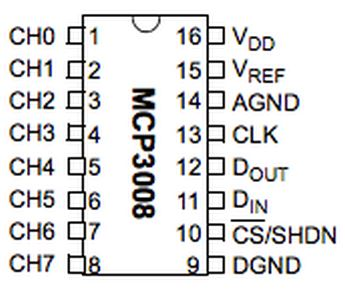
\includegraphics[scale=0.7]{mcp.jpg}
		\centering
		\caption{MCP3008}
	\end{figure}
MCP3008 is a 16 pin IC.	
\begin{enumerate}
\item Digital Ground (DGND): \newline Digital ground connection to internal digital circuitry.
\item Analog Ground (AGND):  \newline Analog ground connection to internal analog circuitry.
\item Analog inputs (CH0 - CH7): \newline Analog inputs for channels 0 - 7, respectively, for the multiplexed inputs. Each pair of channels can be programmed to be used as two independent channels in single-ended mode or as a single pseudo differential input where one channel is IN+ and one channel is IN.
\item Serial Clock (CLK): \newline The SPI clock pin is used to initiate a conversion and clock out each bit of the conversion as it takes place.
\item  Serial Data Input (DIN): \newline The SPI port serial data input pin is used to load channel configuration data into the device.
\item Serial Data Output (DOUT): \newline The SPI serial data output pin is used to shift out the results of the A/D conversion. Data will always change on the falling edge of each clock as the conversion takes place.
\item Chip Select/Shutdown (CS/SHDN): \newline The CS/SHDN pin is used to initiate communication with the device when pulled low. When pulled high, it will end a conversion and put the device in low-power standby. The CS/SHDN pin must be pulled high between conversions.
\end{enumerate}

\subsection{Serial Communication:}
Communication with the 3008 devices is accomplished using a standard SPIcompatible serial interface. 
\begin{itemize}
\item Initiating communication with either device is done by bringing the CS line low .If the device was powered up with the CS pin low, it must be brought high and back low to initiate communication. 
\item The first clock received with CS low and DIN high will constitute a start bit. 
\item The SGL/DIFF bit follows the start bit and will determine if the conversion will be done using single-ended or differential input mode. 
\item The next three bits (D0, D1 and D2) are used to select the input channel configuration. Table shows the bit configuration. 
\item The device will begin to sample the analog input on the fourth rising edge of the clock after the start bit has been received. The sample period will end on the falling edge of the fifth clock following the start bit.
\item  On the falling edge of the 5th clock, the device will output a low null bit. The next 10 clocks will output the result of the conversion with MSB first.
\end{itemize}
	\begin{figure}[h!]
		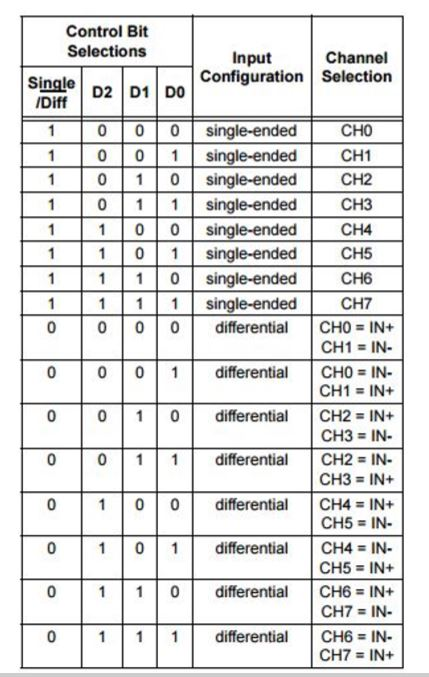
\includegraphics[scale=0.7]{1.jpg}
		\centering
		\caption{Table for bit configuration}
	\end{figure}
		\begin{figure}[h!]
			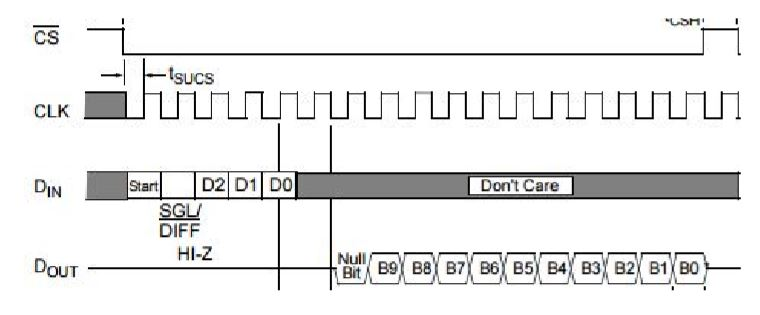
\includegraphics[scale=0.7]{2.jpg}
			\centering
			\caption{Communication with MCP 3008}
		\end{figure}
\subsection{Using the MCP 3008 with the microcontroller SPI ports:}
\begin{itemize}
\item With microcontroller SPI ports, it is required to send groups of eight bits. 
\item Communication with the 3008 devices may not need multiples of eight clocks, it will be necessary to provide more clocks than are required. This is usually done by sending leading zeros before the start bit. 
\item As is shown in Figure , the first byte transmitted to the A/D converter contains seven leading zeros before the start bit. 
\item Arranging the leading zeros this way induces the 10 data bits to fall in positions easily manipulated by the MCU.
\end{itemize}
\begin{figure}[h!]
	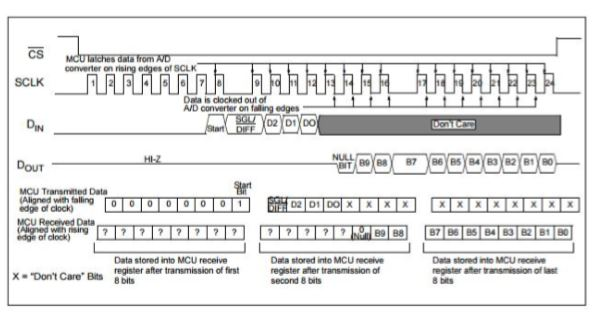
\includegraphics[scale=0.7]{3.jpg}
	\centering
	\caption{SPI Communication with MCP 3008 using 8-bit segments}
\end{figure}
	

\newpage	
\section{Experiment}
\subsection{Interfacing an ADC with RPi using LM35(Temperature Sensor)}
\newpage
		\begin{figure}[h!]
		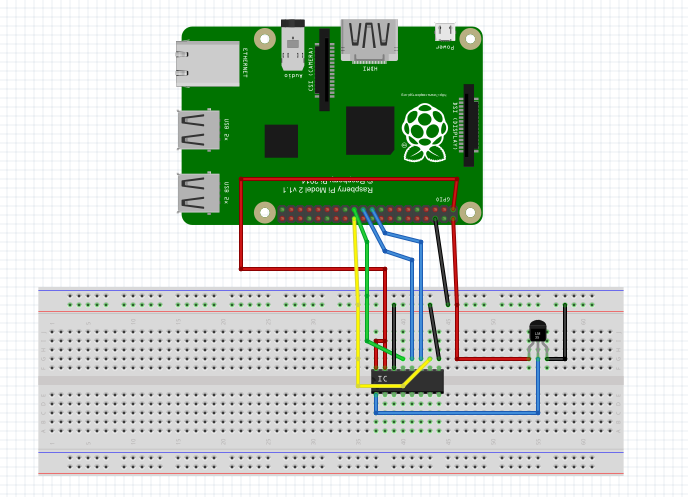
\includegraphics[scale=0.7]{lm35_interfacing.jpg}
		\centering
		\caption{Circuit on Bread Board}
		\end{figure}
	\begin{itemize}
	\item The pin connections are shown in the Circuit above. 
	\item  Here I have used a single ADC MCP3008 interfaced with RPi to which a Lm35 is connected.
	\end{itemize} 
	\textbf{Code}
	\vspace{0.3cm}
	\lstinputlisting[language=Python]{lm35_adc.py}
		
\subsection{Interfacing an ADC with RPi using a Sharp IR Sensor}
        \begin{figure}[h!]
		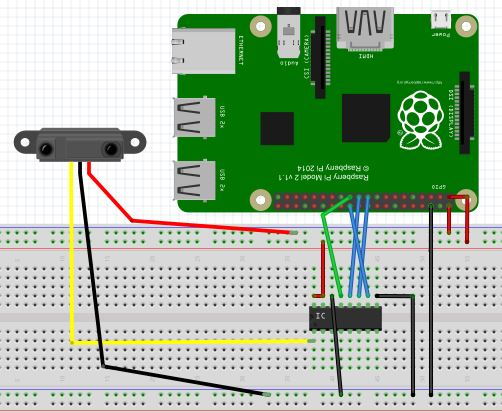
\includegraphics[scale=0.7]{ckt.jpg}
		\centering
        \caption{Circuit on Bread Board}
        \end{figure}
  \begin{itemize}
  \item The pin connections are shown in the Circuit above.
  \item The Connections are showed in the Circuit Schematic in the following figure.
  \item Here I have used a single ADC MCP3008 interfaced with RPi to which a Sharp IR Sensor is connected.
  \end{itemize}

\newpage
\subsection{Circuit Schematic}
        \vspace{3cm}
        \begin{figure}[h!]
		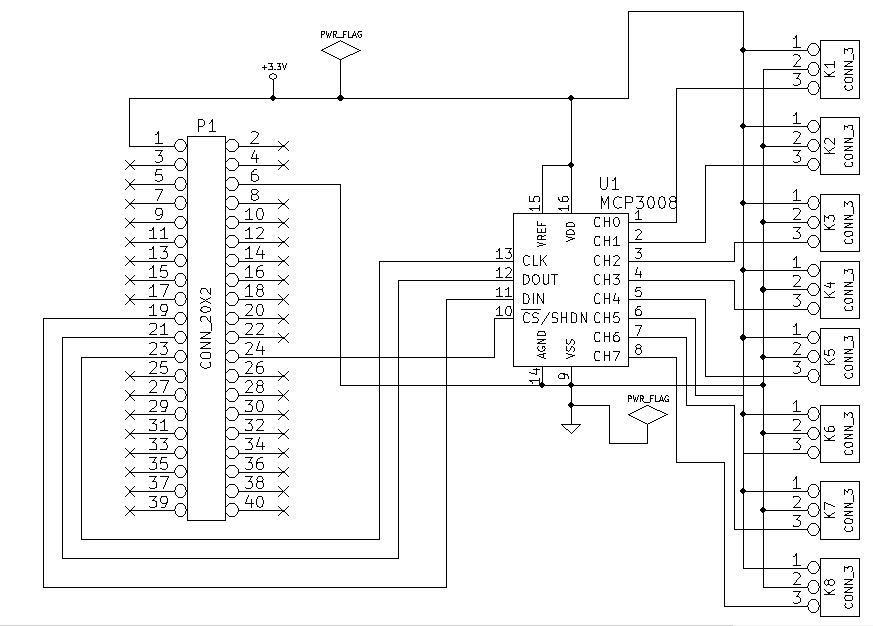
\includegraphics[scale=0.6]{ckt_schematic.jpg}
		\centering
        \caption{Circuit Schematic}
        \end{figure}

	\newpage 
	\textbf{Code}
	\vspace{0.3cm}
	
	\lstinputlisting[language=Python]{adc_IR_sensor.py}
	
\newpage	
\section{Exercise}
\subsection{Interfacing 2 ADC's with RPi using Sharp IR Sensors}
\begin{itemize}
  \item The pin connections are shown in the Circuit Schematic.
  \item Here I have used 2 MCP3008 ADC's interfaced with RPi.
  \item In the this experiment I have used Sharp IR Sensor.
  \item 2 ADC's can be interfaced with RPi mainly because of the 2 chip select pins CE0 and CE1 in RPi.
  \end{itemize}
  \subsection{Circuit Schematic}
        \begin{figure}[h!]
		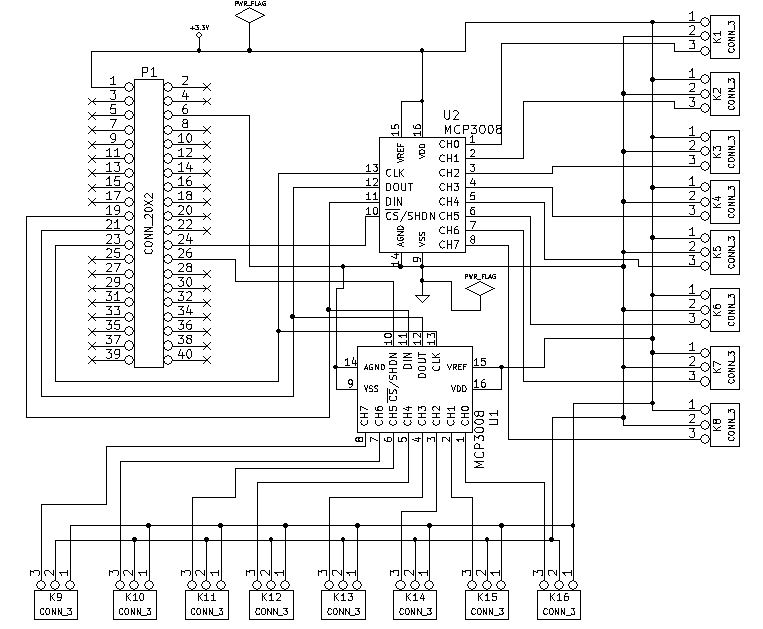
\includegraphics[scale=0.6]{ckt_schematic2.jpg}
		\centering
        \caption{Circuit Schematic}
        \end{figure}

	\newpage 
	\textbf{Code}
	\vspace{0.3cm}
	
	\lstinputlisting[language=Python]{adc2.py}

\section{References}
		\begin{enumerate}
			\item www.raspberrypi-spy.co.ukanalogue-sensors-on-the-raspberry-pi-using-an-mcp3008/
			\item www.en.wikipedia.org/wiki/SerialPeripheralInterface
			\item www.byteparadigm.com/applications/introduction-to-i2c-and-spi-protocols/
			\item developers.google.com/edu/python/
            \item www.alldatasheet.com/Mcp3008+datasheet
		\end{enumerate}	

\end{document}



